\documentclass[UTF8, a4paper, 11pt]{article}
\usepackage[UTF8, scheme=plain]{ctex}
\usepackage{fontspec}
\usepackage{float}
\usepackage{amsmath}
\newtheorem{myDef}{Definition}
\usepackage{graphicx}
\usepackage{geometry}
\usepackage{listings}
\usepackage{xcolor}
\usepackage{caption,subcaption}
\geometry{scale=0.8}
\linespread{1.5}
\usepackage{hyperref}
\usepackage{color}
\usepackage{fontspec}
\usepackage{enumitem}
\usepackage[linesnumbered,boxed]{algorithm2e}    
\usepackage{xeCJK}
\usepackage{indentfirst} 
\graphicspath{{Pic/}} 	% 在于.tex同级的目录下创建名为pic的文件夹,存放图片


\setlength{\parindent}{2em}

\lstset{
    language={C++},
    frame=shadowbox,
    breaklines=true,
    numbers=left,
    backgroundcolor=\color[RGB]{245,245,244},
    rulesepcolor=\color{red!20!green!20!blue!20},
    numberstyle={\color[RGB]{0,192,192}\tiny},
    basicstyle=\footnotesize \fontspec{Source Code Pro}
}
\setenumerate[1]{itemsep=0pt,partopsep=0pt,parsep=\parskip,topsep=0pt}
\setitemize[1]{itemsep=0pt,partopsep=0pt,parsep=\parskip,topsep=0pt}
\setdescription{itemsep=0pt,partopsep=0pt,parsep=\parskip,topsep=0pt}


\title{	
\normalfont \normalsize
\textsc{School of Data and Computer Science, Sun Yat-sen University} \\ [25pt] %textsc small capital letters
\rule{\textwidth}{0.5pt} \\[0.4cm] % Thin top horizontal rule
\huge 光线追踪\\ % The assignment title
\rule{\textwidth}{2pt} \\[0.5cm] % Thick bottom horizontal rule
\author{18308045 谷正阳, 18340014 陈嘉宁, 18340197 叶靖云}
\date{\normalsize\today}
}

\begin{document}
\maketitle
\tableofcontents
\newpage
\section{Abstract}
本文将介绍光追的一些原理,并展示最后结果。更加详细的每个人的工作详见小组报告。
\section{光追中随机数的应用}
光线追踪与渲染管线相比,比较真实地描绘了成像的物理过程,但在其中也引用了一些随机数来简化一些物理过程。
\subsection{抗锯齿}
光线追踪生成图像本质是位图,当图像像素数量比较少时,锯齿会非常明显。因此需要模糊化处理来减少锯齿。具体操作是对于每一个像素,以它所在的一个2x2的方格中均匀分布随机取样若干次,分别计算
颜色再取平均:
\begin{lstlisting}
color pixel_color(0.0f, 0.0f, 0.0f);
for (int s = 0; s < samples_per_pixel; ++s) {
	float u = float(i + random_float(local_rand_state)) / (image_width - 1);
	float v = float(j + random_float(local_rand_state)) / (image_height - 1);
	ray r = (*cam)->get_ray(u, v, local_rand_state);
	pixel_color += ray_color(r, background, world, max_depth, local_rand_state);
}
write_color(fb + pixel_index * 3, pixel_color, samples_per_pixel);
\end{lstlisting}
\begin{lstlisting}
__device__ void write_color(int *ib, color pixel_color, int samples_per_pixel) {
    float r = pixel_color.x();
    float g = pixel_color.y();
    float b = pixel_color.z();

    // Divide the color by the number of samples and gamma-correct for gamma=2.0.
    float scale = 1.0f / samples_per_pixel;
    r = sqrt(scale * r);
    g = sqrt(scale * g);
    b = sqrt(scale * b);

    // Write the translated [0,255] value of each color component.
    ib[0] = static_cast<int>(256 * clamp(r, 0.0f, 0.999f));
    ib[1] = static_cast<int>(256 * clamp(g, 0.0f, 0.999f));
    ib[2] = static_cast<int>(256 * clamp(b, 0.0f, 0.999f));
}
\end{lstlisting}
这样如果采样数够多,采样会很均匀,相当于将1x1的像素模糊成了2x2的像素,在图形边缘处点比较稀疏会颜色浅,在图形内部点比较稠密会颜色深,就做到了抗锯齿的效果。
\begin{figure}[H]
    \centering
    
\includegraphics[width=0.8\textwidth]{antialias.png}
    \caption{Before and after antialiasing}
\end{figure}
\subsection{漫反射}
现实中的漫反射其实也是一种镜面反射,只不过由于物体表面粗糙,微观上看表面上不平滑的小平面很多导致小区域内法向量会急剧变化。因而从宏观上看,反射方向是随机的。但是在计算机实现中,真正去
实现不光滑的平面是非常困难的。Lambertian散射是一种模拟宏观反射的模型,它假设在任意一个小平面内的法向量分布是均匀分布的,因而朝所有夹角小于$\pi$的方向反射的概率相同。实现上,是在与
平面相切的半径为1的小球表面随机取样,击中点到该点的方向设为反射方向:
\begin{lstlisting}
vec3 scatter_direction = rec.normal + random_unit_vector(local_rand_state);

// Catch degenerate scatter direction
if (scatter_direction.near_zero())
    scatter_direction = rec.normal;

scattered = ray(rec.p, scatter_direction, r_in.time());
\end{lstlisting}
\begin{figure}[H]
    \centering
    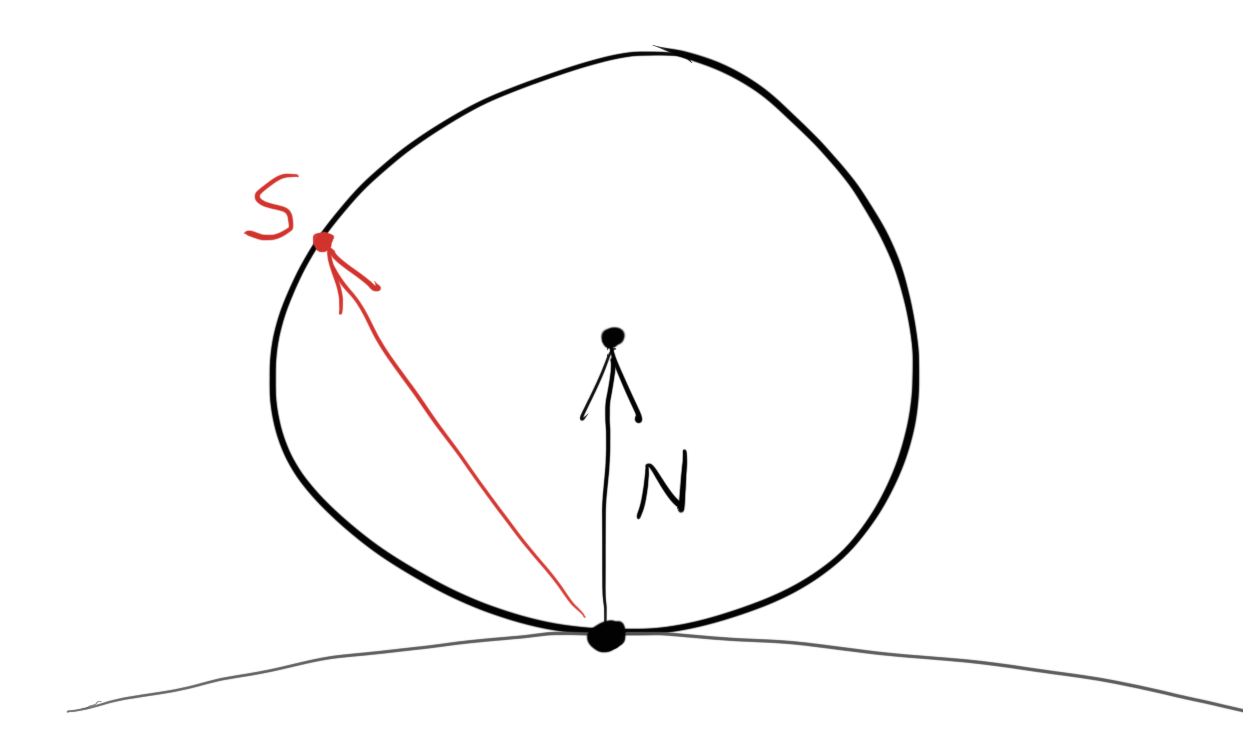
\includegraphics[width=0.8\textwidth]{rand-unitvec.png}
    \caption{Generating a random unit vector}
\end{figure}
\subsection{模糊反射}
模糊反射实际上是镜面反射和Labertian散射之间的状态,它是在镜面反射方向上再加一个方向随机长度为fuzz的一个向量:
\begin{figure}[H]
    \centering
    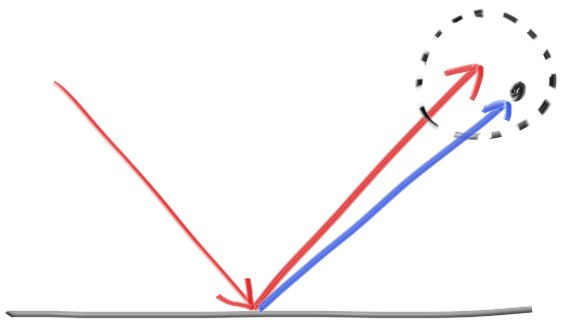
\includegraphics[width=0.8\textwidth]{reflect-fuzzy.jpg}
    \caption{Generating fuzzed reflection rays}
\end{figure}
当fuzz很小时该随机向量可以忽略不计,就是镜面反射;当fuzz很大时,原先计算的镜面反射方向可与忽略不计,此时就是漫反射。
\subsection{透明材质}
现实生活中的透明材质(如水面),并不是只有折射的。除了内部光线的全反射,外部光线在某些角度上也是会产生反射的,而且越接近一个陡峭的角度就越容易反射:
\begin{figure}[H]
    \centering
    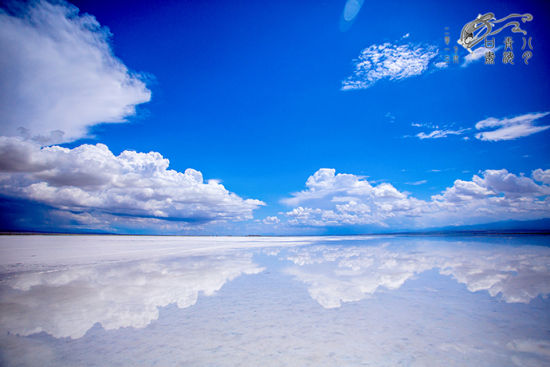
\includegraphics[width=0.8\textwidth]{茶卡盐湖.jpg}
    \caption{茶卡盐湖}
\end{figure}
这一特点用Schlick Approximation
来描述,同样用到了随机数:
\begin{lstlisting}
if (cannot_refract || reflectance(cos_theta, refraction_ratio) > random_float(local_rand_state))
    direction = reflect(unit_direction, rec.normal);
else
    direction = refract(unit_direction, rec.normal, refraction_ratio);
\end{lstlisting}
\subsection{光圈}
现实中的摄像头光线并非汇聚于一点,而是有一个有大小的光圈:
\begin{figure}[H]
    \centering
    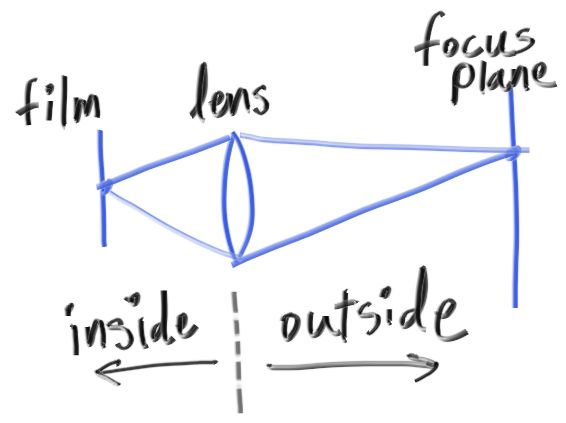
\includegraphics[width=0.8\textwidth]{cam-lens.jpg}
    \caption{Camera lens model}
\end{figure}
因而光追计算时光线的原点需要遍布一个圆盘,而非只有一个点。为了简化计算,这里并没有采用遍历点的方式,而是在光圈范围内均匀地随机取样一些点作为原点:
\begin{lstlisting}
__device__ ray get_ray(float s, float t, curandState* local_rand_state) const {
    vec3 rd = lens_radius * random_in_unit_disk(local_rand_state);
    vec3 offset = u * rd.x() + v * rd.y();

    return ray(
        origin + offset,
        lower_left_corner + s*horizontal + t*vertical - origin - offset,
        ...
    );
}
\end{lstlisting}
\subsection{动态模糊}
现实中的摄像头是有曝光时间的,并非捕捉瞬间的图像,因而运动中的物体会呈现模糊的效果:
\begin{figure}[H]
    \centering
    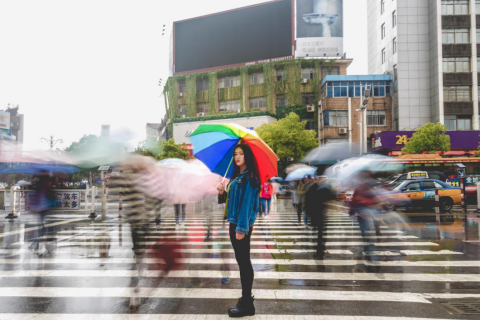
\includegraphics[width=0.8\textwidth]{motion_blur.png}
    \caption{Motion Blur}
\end{figure}
为了简化计算,这里同样没有采取遍历时间点的方法,而是随机采样一些时间点计算并叠加这些不同时刻的图像:
\begin{lstlisting}
__device__ ray get_ray(float s, float t, curandState* local_rand_state) const {
    ...
    return ray(
        origin + offset,
        lower_left_corner + s*horizontal + t*vertical - origin - offset,
        random_float(time0, time1, local_rand_state)
    );
}
\end{lstlisting}
\section{结果展示}
在没有加入动态模糊的情况下最终渲染得到的图像如下:
\begin{figure}[H]
    \centering
    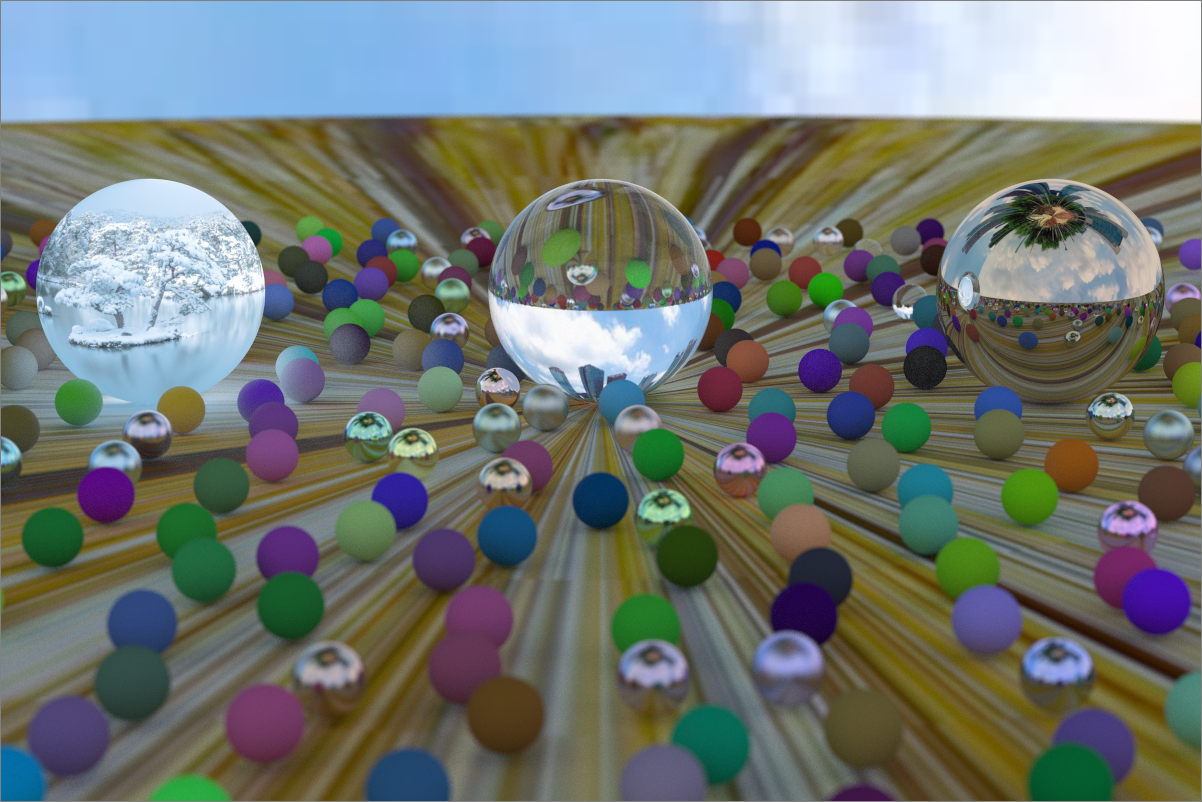
\includegraphics[width=12cm]{Pic/result.png}
\end{figure}
而加入动态模糊后最终渲染得到的图像如下:
\begin{figure}[H]
    \centering
    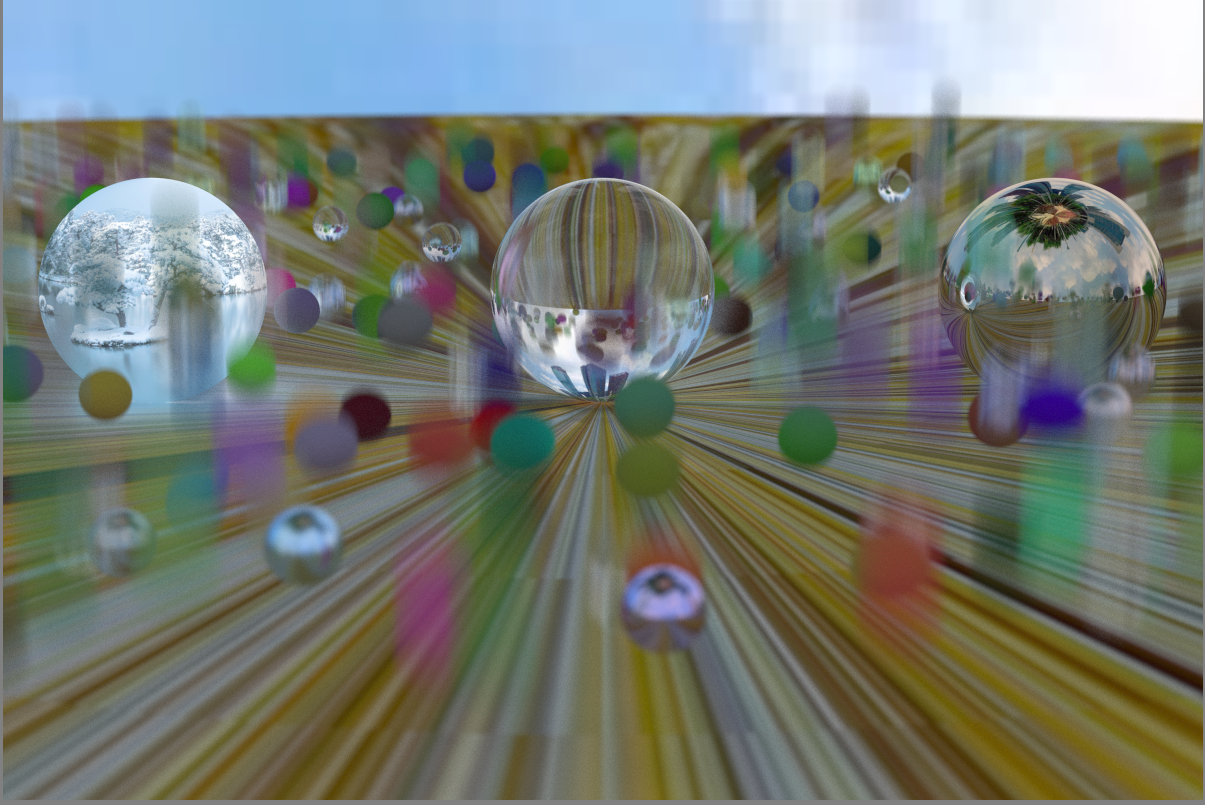
\includegraphics[width=12cm]{Pic/result_moving.png}
\end{figure}
同时我们制作了一个逐帧动画(具体制作过程还请参照个人报告的内容),动画已经以GIF格式随文件一同上传。
%\clearpage
%\bibliography{E:/Papers/LiuLab}
%\bibliographystyle{apalike}
\end{document}
%%% Local Variables:
%%% mode: latex
%%% TeX-master: t
%%% End:
